\documentclass[11pt]{article}
\usepackage{amsmath,amssymb,amsthm,graphicx,geometry,hyperref}
\geometry{margin=1in}
\newtheorem{theorem}{Theorem}[section]
\newtheorem{proposition}[theorem]{Proposition}
\newtheorem{lemma}[theorem]{Lemma}
\newtheorem{definition}[theorem]{Definition}
\title{A Certified Stationary-Orbit Bifurcation for a Cone-Volume-Weighted Radial--Normal Angle on Prolate Spheroids}
\author{Katsushi Furuta\\Independent Researcher}
\date{September 5, 2026}
\begin{document}
\maketitle
\begin{abstract}
We study a cone-volume-weighted radial--normal angle functional with the base point as the variable and prove that its stationary set changes topology along the one-parameter family of prolate spheroids. Rotational symmetry forces the center to remain stationary, while on one side of a critical axis ratio there is a stationary circle in the equatorial plane that shrinks into the center at the critical parameter. A local analytic reduction expresses the bifurcation through an equatorial quadratic coefficient $Q(a)$, a quartic coefficient $H_4(a)$, and an axial quadratic coefficient $Q_z(a)$. Rigorous Arb/Acb ball arithmetic certifies a unique simple zero
\[
4.72438340452113340672<a_c<4.72438340452113340673,
\]
with $Q'(a_c)<0$, $H_4(a_c)<0$, and $Q_z(a)>0$ on $[4.7,4.75]$. The resulting stationary circle satisfies $r(a)\to0$ as $a\uparrow a_c$. The computer-assisted part is reproducible from a public twelve-object, SHA-256-pinned certificate chain; symbolic audits independently connect the analytic kernel $h(x)=\arccos^2x$ to the regularized ${}_0F_1$ derivative formulas and to the raw axial kernel. Thus the experimental discovery, analytic reduction, and rigorous interval proof are separated explicitly.
\end{abstract}
\noindent\textbf{Keywords.} stationary orbit; bifurcation; prolate spheroid; cone-volume measure; radial--normal angle; interval arithmetic; computer-assisted proof; experimental mathematics.

\section{Introduction}
We treat the base point of a geometric functional as a variable and ask how its stationary set changes when the underlying body is deformed. Classical center constructions usually select a point. Once uniqueness is lost, however, continuous symmetry can force positive-dimensional stationary sets. The present example makes this mechanism explicit and rigorous.

For a prolate spheroid of polar-to-equatorial axis ratio $a$, numerical exploration first indicated an equatorial stationary circle that contracts toward the center as $a$ approaches a value near $4.72438$. The experiment suggested a local bifurcation governed by a sign change of the transverse quadratic coefficient. We then replaced the exploratory computation by a computer-assisted proof: symbolic kernel audits, rigorous ball-arithmetic integration, a 20-decimal endpoint sign certificate, and a separate axial positivity certificate. This progression from experiment to theorem is the main computational narrative of the paper and is consistent with the role of reproducible computer experiments in experimental mathematics \cite{BorweinBailey}.

The result is local. We prove the existence and local uniqueness of the stationary circle near the center and the change in the local stationary-set labels. We do not claim a global enumeration of every stationary component for every axis ratio.

\section{Basepoint bifurcation}
Let $P$ be a basepoint space, $\Lambda$ a parameter space, and $E_\lambda:P\to\mathbb R$ a family of functionals. Set
\[
\mathcal S=\{(\lambda,p):d_pE_\lambda=0\},\qquad \pi:\mathcal S\to\Lambda.
\]
We label each local stationary component by its dimension, normal Morse index, nullity, and isotropy type.

\begin{definition}[Local basepoint bifurcation]
A point $(\lambda_0,p_0)\in\mathcal S$ is a local basepoint bifurcation point if, for every sufficiently small two-sided neighborhood $I\ni\lambda_0$ and neighborhood $U\ni p_0$, the restricted projection $\pi:\mathcal S\cap(I\times U)\to I$ admits no local trivialization preserving these labels.
\end{definition}

This definition concerns the germ of the stationary set and therefore does not require a global classification away from $(\lambda_0,p_0)$.

\section{Cone-volume-weighted radial--normal angle}
Let $K\subset\mathbb R^3$ be a smooth convex body and $p\in\operatorname{int}K$. For $x\in\partial K$ with outward unit normal $\nu_K(x)$ define
\[
\alpha_{K,p}(x)=\arccos\!\left(\frac{(x-p)\cdot\nu_K(x)}{|x-p|}\right),
\qquad
d\mu_{K,p}(x)=\frac{(x-p)\cdot\nu_K(x)}{3\operatorname{Vol}(K)}\,dA(x),
\]
and
\[
E_K(p)=\int_{\partial K}\alpha_{K,p}(x)^2\,d\mu_{K,p}(x).
\]
The divergence theorem gives $\int_{\partial K}(x-p)\cdot\nu_K\,dA=3\operatorname{Vol}(K)$, so $\mu_{K,p}$ is a probability measure. Cone-volume measure is natural in convex geometry \cite{BoroczkyHenk,BLYZ,HLYZ}; related center constructions include radial and generalized centers \cite{HMP,Moszynska,OHara,Sakata}.

\begin{proposition}[Similarity invariance]\label{prop:similarity}
If $T(x)=sUx+q$ with $s>0$ and $U\in O(3)$, then $E_{T(K)}(T(p))=E_K(p)$.
\end{proposition}
The angle is similarity invariant, while the support-distance factor, area element, and volume scale by $s$, $s^2$, and $s^3$, respectively. Hence the normalized measure is invariant. In particular, signs, Morse indices, and nullities of the basepoint Hessian are unchanged by uniform rescaling. We therefore normalize the equatorial semiaxis to one below.

\section{Prolate spheroids and local reduction}
Consider
\[
K_a=\{(x,y,z):x^2+y^2+z^2/a^2\le1\},\qquad a\ge1.
\]
The symmetry group contains rotations about the $z$ axis and reflection in the equatorial plane. The center is stationary for every $a$. On $z=0$, reflection symmetry forces $\partial_zE_a=0$, and the remaining equation depends only on $r=(x^2+y^2)^{1/2}$.

Near the center,
\[
E_a(r)=E_a(0)+\frac{Q(a)}2r^2+\frac{H_4(a)}{24}r^4+O(r^6),
\]
so
\[
\partial_rE_a(r)=rG(a,r^2),\qquad
G(a,s)=Q(a)+\frac{H_4(a)}6s+O(s^2).
\]
The functions are real analytic near the parameter range considered here.

\section{Experimental discovery and certification design}
Exploratory high-precision computations were used only to locate the candidate sign change and to identify the coefficients that should control the local branch. They are not proof objects. The proof stage fixes closed parameter intervals, analytic formulas, outward-rounded Arb/Acb arithmetic, and fail-closed sign conditions.

The certificate architecture separates three questions. First, symbolic audits check the equatorial quadratic and quartic kernels. Second, a rigorous interval certificate establishes the sign change and monotonicity of $Q$ and the negativity of $H_4$. Third, the axial calculation is independently audited and certified, preventing an equatorial stationary point from escaping the three-dimensional stationary condition. A separate symbolic audit verifies the regularized ${}_0F_1$ derivative chain used by the interval kernels.

\section{Certified critical axis ratio}
\begin{proposition}[Certified local coefficients]\label{prop:certified}
On $[4.7,4.75]$ there is a unique $a_c$ satisfying $Q(a_c)=0$, and
\[
4.72438340452113340672<a_c<4.72438340452113340673.
\]
Moreover $Q'(a_c)<0$ and $H_4(a_c)<0$.
\end{proposition}
The endpoint enclosures are
\[
Q(4.72438340452113340672)\in[4.45950117779900917098986772,4.45950117779900917098986968]\times10^{-22},
\]
\[
Q(4.72438340452113340673)\in[-5.00431892402172225190109006,-5.00431892402172225190108810]\times10^{-22}.
\]
On the five subintervals $[4.70,4.71],\ldots,[4.74,4.75]$, the certified enclosures for $Q'$ are respectively
\[
[-0.10545,-0.08573],\ [-0.10492,-0.08527],\ [-0.10438,-0.08480],\ [-0.10386,-0.08434],\ [-0.10333,-0.08388],
\]
and those for $H_4$ are
\[
[-1.49670,-1.39252],\ [-1.49333,-1.38959],\ [-1.48998,-1.38666],\ [-1.48664,-1.38375],\ [-1.48331,-1.38085].
\]
Thus the zero is simple and unique on the stated interval.

The analytic implicit-function theorem applied to $G(a,s)=0$ gives a unique local branch $s(a)$ with $s(a_c)=0$ and
\[
s'(a_c)=-\frac{6Q'(a_c)}{H_4(a_c)}<0.
\]
Hence $s(a)>0$ for $a<a_c$ sufficiently close to $a_c$, and the stationary radius $r(a)=\sqrt{s(a)}$ satisfies $r(a)\to0$ as $a\uparrow a_c$. The coefficient $c=6Q'(a_c)/H_4(a_c)$ is rigorously enclosed by $[0.3415,0.4516]$; the value $0.39474123$ is only a non-certified reference-point estimate.

\begin{figure}[ht]
\centering
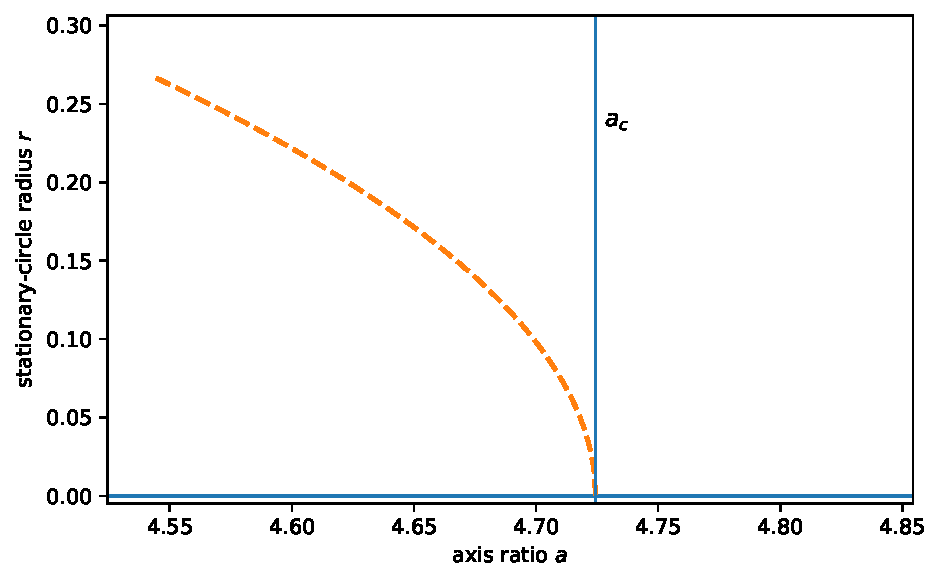
\includegraphics[width=.82\linewidth]{fig1_local_bifurcation.pdf}
\caption{Certified local bifurcation picture. The dashed curve represents the leading law $r_*(a)^2=c(a_c-a)$. The coefficient satisfies the certified enclosure $c\in[0.3415,0.4516]$; $0.39474123$ is a non-certified reference-point estimate. The figure is schematic, not a global numerical continuation.}
\label{fig:bifurcation}
\end{figure}

\section{Axial confinement and the stationary circle}
Write the axial derivative near the center as
\[
\partial_zE_a(x,y,z)=zH(a,x,y,z^2).
\]
Real analyticity implies continuity of $H$. The certified axial coefficient satisfies
\[
Q_z(a)>0\quad\text{for all }a\in[4.7,4.75],
\]
with rigorous lower bound $0.0885587746621582$. Since $H(a_c,0,0,0)=Q_z(a_c)>0$, continuity gives $H>0$ in a sufficiently small neighborhood of $(a_c,0)$. Thus $\partial_zE_a=0$ forces $z=0$ there.

Consequently the nonzero equatorial solution produces a stationary circle $C_a\cong S^1$. The radial normal eigenvalue is negative. The axial eigenvalue remains positive on $C_a$ for $a<a_c$ sufficiently close to $a_c$, by $Q_z(a_c)>0$, $r(a)\to0$, and continuity of the Hessian. The tangential zero eigenvalue is forced by rotational symmetry. Hence $C_a$ is locally Morse--Bott.

\section{Main theorem}
\begin{theorem}[Certified stationary-orbit bifurcation]\label{thm:main}
For the cone-volume-weighted radial--normal angle functional on $K_a$, $(a_c,0)$ is a local basepoint bifurcation point. In a sufficiently small neighborhood of the center,
\[
\operatorname{Crit}(E_a)=\{0\}\sqcup C_a\quad(a<a_c),
\]
where $C_a\cong S^1$ and $r(a)\to0$ as $a\uparrow a_c$; at $a=a_c$ the equatorial part of the center Hessian has nullity two; and for $a>a_c$ sufficiently close to $a_c$ the only local stationary component is the center. Therefore the local stationary-set projection is not label-preserving locally trivial across $a_c$.
\end{theorem}

\section{Endpoint regularization}
The direct $\arccos^2$ representation is poorly conditioned for numerical differentiation near an endpoint. Set
\[
\beta=\arctan((a-a^{-1})\sin\theta\cos\theta),\qquad z=\beta^2,
\]
and define
\[
S={}_0F_1(;3/2;-z/4),\quad T={}_0F_1(;5/2;-z/4),\quad U={}_0F_1(;7/2;-z/4),\quad V={}_0F_1(;9/2;-z/4).
\]
For $h(x)=\arccos^2x$, the derivatives used by the interval kernels are represented by
\[
h_1=-\frac2S,\qquad h_2=\frac{2T}{3S^3},
\]
\[
h_3=\frac{2U}{15S^4}-\frac{2T^2}{3S^5},\qquad
h_4=\frac{2V}{105S^5}-\frac{4UT}{9S^6}+\frac{10T^3}{9S^7}.
\]
At $\beta=0$ these formulas are interpreted by analytic continuation through the entire ${}_0F_1$ representations, with $S(0)=1$. On the target interval $S=\sin\beta/\beta$ has a positive lower bound, so the denominators remain uniformly separated from zero. This regularization is what permits rigorous resolution of endpoint sign margins of order $5\times10^{-22}$. The four identities above are themselves checked by an independent symbolic audit, with all four differences simplifying exactly to zero.

\section{Reproducibility and proof objects}
The proof archive contains twelve SHA-256-pinned objects under \texttt{CERTIFICATES/prolate/local\_bifurcation/}. They comprise the cap-chain certificate and reports, the symbolic audits for the equatorial kernels, the 20-decimal $a_c$ certificate and JSON report, the raw-kernel $Q_z$ symbolic audit, the $Q_z$ Arb certificate and JSON report, and the ${}_0F_1$ derivative-chain symbolic audit. Running \texttt{sha256sum -c SHA256SUMS.txt} gives 12/12 OK at the canonical commit
\[
\texttt{abf704b8701f3da8eb41d8a99408570a413b2214}.
\]
The $a_c$ run uses Python 3.13.14, 100 decimal digits, and tolerance $10^{-40}$. The $Q_z$ run uses Python 3.13.14, 70 decimal digits, tolerance $10^{-28}$, and five parameter subdivisions. Recorded common components include python-flint 0.9.0, FLINT 3.6.0, SymPy 1.14.0, and mpmath 1.3.0.

The $Q_z$ certificate gates the manuscript claim itself: \texttt{status=CERTIFIED} requires both positivity on all five parameter intervals and \texttt{worst\_lower >= 0.0885587746621582}. The symbolic $Q_z$ audit differentiates the raw weighted kernel twice while keeping $h$ abstract; it does not depend on a pre-substituted finite Taylor jet.

\section{Scope and relation to center theory}
The result concerns a local germ, not a global classification. Interval continuation machinery for global component tracking is therefore not a premise of Theorem~\ref{thm:main}. The novelty is also not a new abstract $O(2)$ bifurcation theorem. Rather, it is the rigorous realization of a positive-dimensional stationary orbit and its collapse in a concrete convex-geometric functional, with the experimental and certified stages exposed separately.

Classical work on selectors, radial centers, and generalized centers emphasizes distinguished points \cite{HMP,Moszynska,OHara,Sakata}. Here the loss of uniqueness is itself informative: symmetry turns an off-axis stationary point into an orbit, and the orbit becomes the geometric carrier of the bifurcation.

\section{Conclusion}
A computational experiment on prolate spheroids led to a candidate stationary-circle bifurcation. Symbolic reduction and rigorous interval arithmetic convert that observation into a theorem: a unique critical axis ratio is certified to twenty decimal places, a stationary circle exists on one side and contracts to the center, and axial positivity closes the three-dimensional stationary condition. The public certificate chain makes the numerical part independently repeatable and distinguishes exploratory evidence from proof objects.

\section*{Data and code availability}
All computer-assisted proof objects used in this article are publicly archived in the Basepoint Geometry repository \cite{Repo}. The canonical proof state is commit \texttt{abf704b8701f3da8eb41d8a99408570a413b2214}; its local-bifurcation manifest contains twelve SHA-256-pinned objects and verifies 12/12. The separate \texttt{bg-prolate-spheroid} repository is diagnostic only and is not evidence for the theorem.

\begin{thebibliography}{99}
\bibitem{BoroczkyHenk} K. J. B\"or\"oczky and M. Henk, Cone-volume measure of general centered convex bodies, \emph{Adv. Math.} 286 (2016), 703--721.
\bibitem{BLYZ} K. J. B\"or\"oczky, E. Lutwak, D. Yang, and G. Zhang, The logarithmic Minkowski problem, \emph{J. Amer. Math. Soc.} 26 (2013), 831--852.
\bibitem{HLYZ} Y. Huang, E. Lutwak, D. Yang, and G. Zhang, Geometric measures in the dual Brunn--Minkowski theory and their associated Minkowski problems, \emph{Acta Math.} 216 (2016), 325--388.
\bibitem{HMP} I. Herburt, M. Moszy\'nska, and Z. Peradzy\'nski, Remarks on radial centres of convex bodies, \emph{Math. Phys. Anal. Geom.} 8 (2005), 157--172.
\bibitem{Moszynska} M. Moszy\'nska, Looking for selectors of star bodies, \emph{Geom. Dedicata} 83 (2000), 131--147.
\bibitem{OHara} J. O'Hara, Renormalization of potentials and generalized centers, \emph{Adv. Appl. Math.} 48 (2012), 365--392.
\bibitem{Sakata} S. Sakata, Stationary radial centers and symmetry of convex polytopes, \emph{Colloq. Math.} 159 (2020), 91--106.
\bibitem{BorweinBailey} J. M. Borwein and D. H. Bailey, \emph{Mathematics by Experiment: Plausible Reasoning in the 21st Century}, A K Peters, 2004.
\bibitem{Repo} K. Furuta, Basepoint Geometry: computational certificates for the prolate-spheroid basepoint bifurcation, software and proof archive, GitHub, canonical commit \texttt{abf704b8701f3da8eb41d8a99408570a413b2214}, 2026. \url{https://github.com/cotaxxxx/basepoint-geometry}.
\end{thebibliography}
\end{document}
